% --- Dokumententyp ---
% Dokumententyp scrreprt; deutsch, doppelseitig mit 1cm Bindekorrektur
\documentclass[BCOR=1cm, twoside, ngerman]{scrreprt}

% --- Präambel ---
% Erweiterungen einbinden
\usepackage[utf8]{inputenc}
\usepackage{babel}
\usepackage{biblatex}
\usepackage{cleveref}
\usepackage[multiple]{footmisc}
\usepackage{graphicx}
\graphicspath{{imgs/}}
\usepackage{csquotes}

% um zeilenumbrüche in Tabellen zu erstellen
\usepackage{makecell}

% für subfigure:
\usepackage{caption}
\usepackage{subcaption}

% tikz pakete für die Erstellung von plots:
\usepackage{tikz}
\usepackage{tikz-timing} % für timing-diagramme:

% für svg bilder:
\usepackage{svg}

% formatierung von code im text:
\newcommand{\code}[1]{\texttt{#1}}
% low-activ Signal:
\newcommand{\lowactive}[1]{$\overline{\code{#1}}$}

% Attribute für die Titelseite
\titlehead{\hfill
\includegraphics[width=4cm]{logo.png}} % Das FH-Logo
\subject{Fachhochschule Bielefeld\\Fachbereich Ingenieurwissenschaften und Mathematik\\Studiengang Ingenieurinformatik}
\title{Titel der Ausarbeitung}
\subtitle{Art der Ausarbeitung}
\author{Name der/s Autors/in bzw. Autoren/innen inkl. Matrikelnummer}
\date{\today} % Das Datum der Abgabe
\publishers{Betreuer:\\ Prof. Dr. Axel Schneider\\Dr. Hanno Gerd Meyer}

% Pfad zur bib-Datei mit Literaturquellen
\bibliography{references.bib}

% --- Dokumentenrumpf ---
\begin{document}
% Titelseite erstellen
\maketitle

% Deutsche und englische Zusammenfassung in abstract-Umgebung
\begin{abstract}
Eine kurze deutsche Zusammenfassung.\\

A short abstract in english.
\end{abstract}

% Erstelle Inhaltsverzeichnis
\tableofcontents
% Quellenverzeichnis setzen, welches im Inhaltsverzeichnis als Kapitel erscheinen soll. Der Titel soll 'Literaturverzeichnis' sein.
\printbibliography[heading=bibintoc, title={Literaturverzeichnis}]

% Einleitung
\chapter[Einleitung]{Einleitung}

Diese Studienarbeit behandelt die Konzipierung und Implementierung eines digitalen Funktionsgenerators in der Hardwarebeschreibungssprache VHDL.
Ein Funktionsgenerator ist ein elektronisches Bauteil, das in der Lage ist, verschiedene Spannungsverläufe an seinem Ausgang auszugeben.
Diese können dann an andere Bauteile angeschlossen und so technisch genutzt werden.
Beispielsweise kann ein Funktionsgenerator eingesetzt werden, um ein Rechteck- oder Sinussignal auszugeben.
Der praktische Nutzen könnte dann die Aktivierung eines Kameraauslösers in einer bestimmten Frequenz oder die Helligkeitssteuerung einer LED sein. \\
Ein Funtkionsgenerator kann als Digitalschaltung in einen Chip integriert oder auf eine Platine gelötet werden, er könnte aber auch als Programm eines Universalrechners laufen.
Softwarelösungen verfügen nicht über das hohe Maß an Effizienz und die Geschwindigkeit einer integrierten Schaltung.
Diese wiederum sind nur in großer Stückzahl rentabel herstellbar.
Von Hand gelötete Schaltungen lassen sich nicht einfach reproduzieren und sind nicht besonders kompakt.
Einen Mittelweg zwischen diesen Zielkonflikten bieten sogenannte ``\textbf{F}ree \textbf{P}rogrammable \textbf{G}ate \textbf{A}rrays'', kurz FPGA.
Auf diesen ICs befinden sich verschiedene Bausteine die durch Anlegen einer Programmierspannung miteinander verknüpft werden können.
Somit ist es möglich, verschiedenste Schaltungen auf demselben IC umzusetzen. \\
Die Schaltungen können mithilfe einer Beschreibungssprache designed werden.
Eine dieser Sprachen ist VHDL (``\textbf{V}ery \textbf{H}ighspeed Hardware \textbf{D}escription \textbf{L}anguage''), welche in dieser Studienarbeit verwendet werden soll.
Die Implementation auf einem FPGA mittels Beschreibungssprache bietet den Vorteil guter Reproduzierbarkeit bei vergleichsweise hoher Konfigurierbarkeit und Effizienz. \\
Bei dem in diesem Projekt verwendeten FPGA handelt es sich um den Artix 7 von Xilinx.
Dieser ist in das Entwicklungsboard Basys 3 des Herstellers digilent eingebettet \cite{digilent2016}.
Es verfügt über diverse Peripheriemodule wie eine UART Schnittstelle, einen micro-USB Anschluss oder einen VGA Ausgang. \\
In dieser Arbeit wird zunächst der konzeptuelle Aufbau des Funktionsgenerators erläutert, dann werden die einzelnen Komponenten, aus denen er besteht, sowie die interne Taktung der Komponenten erläutert.
Schließlich wird noch ein Funktionstest durchgeführt, bei dem die theoretisch erwarteten Resultate den tatsächlichen gegenübergestellt werden. \\
Sämtlicher Quellcode findet sich im GitHub-Repository unter folgender URL: \\
\href{https://github.com/markushart/studienarbeit_function_generator.git}{\code{https://github.com/markushart/studienarbeit\_function\_generator.git}}
% Hauptteil
\chapter{Konzept}
Im Folgenden werden die verschiedenen Funktionsmerkmal des Funktionsgenerators erläutert.
Anschließend wird sein Konzept anhand des grundlegenden Aufbaus des Funktionsgenerators erklärt.
 
\section{Funktionsmerkmale} \label{Concept:Feature}
In diesem Abschnitt wird geschildert, was der Generator leisten kann und wie er sich konfigurieren lässt. 

\subsection{Funktionen} \label{Concept:Feature:Func}
Der Generator kann auf vier verschiedene Funktionsbausteine zurückgreifen, die jeweils einen anderen Spannungsverlauf ausgeben:

\begin{enumerate}
   \item \textbf{Konstante Funktion} \\ 
    Die konstante analoge Spannung \analog{high} liegt am Ausgang an.
  \item \textbf{Rechteck-Funktion} \\
    Der Wert wechselt zwischen \analog{high} und \analog{low} in der Frequenz $f$.
    Der Anteil der Zykluszeit $T$, in dem der Ausgang auf \analog{high} ist, wird über den Parameter dutycycle eingestellt.
    Die Dauer des \analog{high}-Pegels bzw. \analog{low}-Pegels, $T_{h}$ und $T_{l}$ berechnen sich folgendermaßen:
    \begin{align}
      T_{l} &= T \cdot \frac{dutycycle}{255}, dutycycle \in \{0, 1, ..., 255\} \label{Concept:Feature:Func:eqdc1} \\
      T_{h} &= T - T_{l} \label{Concept:Feature:Func:eqdc2}
    \end{align}
    Auf diese Art lassen sich Rechteck-Signale mit einstellbarer Pulsweite erzeugen.
    Diese sogenannten PWM-Signale (``\textbf{P}uls \textbf{W}eiten \textbf{M}odulation'') werden in vielen technischen Anwendungen verwendet.
  \item \textbf{Zick-Zack-Funktion} \\
    Der Analogwert steigt von \analog{low} bis \analog{high} linear an, erreicht er \analog{high}, fällt der Analogwert wieder kontinuierlich auf \analog{low} ab. Somit schwankt der Ausgangspegel mit der Frequenz $f$.
  \item \textbf{Rampen-Funktion} \\
    Der Analogwert wächst, wie bei der Zick-Zack-Funktion, linear bis auf \analog{high} an, danach fällt er aber auf \analog{high} zurück.
    Alternativ kann die Rampe auch von \analog{high} her abfallen und bei Erreichen von \analog{low} wieder auf \analog{high} zurück springen.
\end{enumerate}

\begin{figure}[h] \centering
  {
    \pgfplotsset{
    xtick={0, 15, 30, 45, 60, 75, 90},
    ytick={0, 0.55, 1.1, 1.65, 2.2, 2.75, 3.3},
    xmin=0, xmax=90,
    ymin=-0.2, ymax=3.5,
    % xlabel=$t$,
    xticklabels={$0$, , $T$, , $2T$, , $3T$,}, % \pgfmathprintnumber{\tick}},
    yticklabels={},
    grid=major,
    width=0.52\textwidth,
    height=0.4\textwidth}
  % constant
  \subfloat[][konstante Funktion]{ 
    \begin{tikzpicture}
      \begin{axis}[yticklabels={$h$, , , , , ,$l$}, ylabel=$U(t)$]
        \addplot[color=blue] coordinates{(0, 1.75)(90, 1.75)};
      \end{axis}
    \end{tikzpicture}
    \label{Concept:Plot:const}
  } 
  % square
  \subfloat[][Rechteckfunktion]{
    \begin{tikzpicture}
      \begin{axis}
        \addplot[color=blue]  coordinates{(0, 0)(15, 0)(15, 3.3)(30, 3.3)(30, 0)(45, 0)(45, 3.3)(60, 3.3)(60, 0)(75, 0)(75, 3.3)(90, 3.3)};
      \end{axis}
    \end{tikzpicture}
    \label{Concept:Plot:square}
  } 

  % zigzag \foreach \x in {0, 15, ..., 90} {(\x, 3.3)}
  \subfloat[][Zick-Zack-Funktion]{
    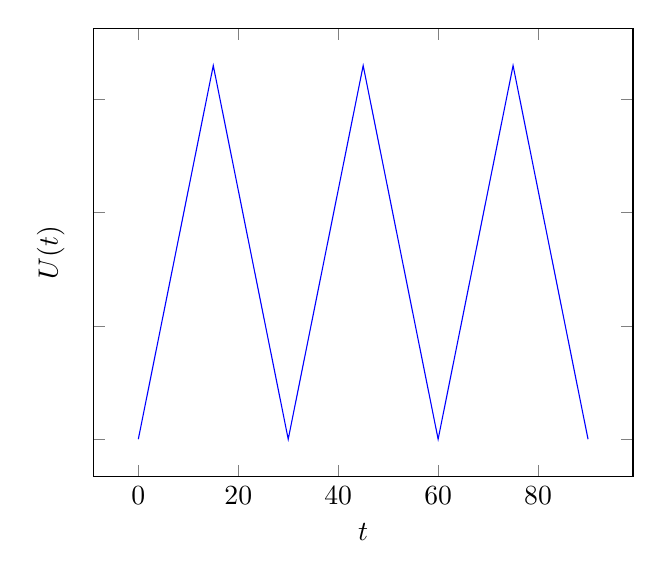
\begin{tikzpicture}
      \begin{axis}[yticklabels={$h$, , , , , ,$l$}, ylabel=$U(t)$, xlabel=$t$]
        \addplot[color=blue] coordinates{(0, 0)(15, 3.3)(30, 0)(45, 3.3)(60, 0)(75, 3.3)(90, 0)};
      \end{axis}
    \end{tikzpicture}
    \label{Concept:Plot:zigzag}
  }
  % ramp
  \subfloat[][Rampenfunktion]{
    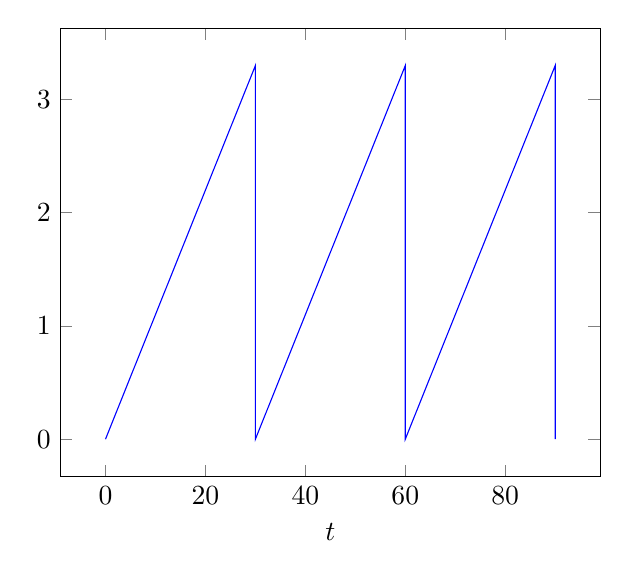
\begin{tikzpicture}
      \begin{axis}[xlabel=$t$]
        \addplot[color=blue, domain=0:90]  coordinates{(0, 0)(30, 3.3)(30, 0)(60, 3.3)(60, 0)(90, 3.3)(90, 0)};
      \end{axis}
    \end{tikzpicture}
    \label{Concept:Plot:ramp}
  }
  \caption{Funktionen, die der Funktionsgenerator ausgeben kann. Ihr Verlauf ist als Spannung $U(t)$ über der Zeit $t$ aufgetragen. Die Zykluszeit und \analog{high} bzw. \analog{low} sind durch  $T$, $h$ und $l$ gekennzeichnet.} \label{Concept:Plot}
\end{figure}

\subsection{Konfiguration}
Der Funktionsgenerator muss, um extern konfiguriert werden zu können, über eine Möglichkeit für Nutzereingaben verfügen.
Zu diesem Zweck wird die UART-Schnittstelle auf dem Basys 3-Board genutzt.
Über diese kann der Nutzer Konfigurationsbefehle per Computer versenden, die dann vom Generator interpretiert werden.
Darüber hinaus nutzerseitig wurde ein Python-Script geschrieben, das die Kommunikation mit dem Generator vereinfacht.

\section{Aufbau}
Der Funktionsgenerator ist aus verschiedenen Einzelkomponenten zusammengesetzt.
Ihre Verschaltung im Generator ist in \cref{Concept:FuncGenDia} zu sehen.
In der Abbildung kann man gut erkennen, dass die verschiedenen Funktionen parallel arbeiten und von der Konfigurationsschnittstelle mit den Signalen \bitvect{cyc\_ticks}, \bitvect{high}, \bitvect{low}, \bitvect{thresh} und \bitvect{direction} gesteuert werden.
Das Signal \bitvect{waveform} steuert den Multiplexer, der das Ausgabesignal \bitvect{y\_out} an die interne Schnittstelle des DAC-Wandlers weitergibt.
Diese Schnittstelle generiert daraus die Signale \lowactive{SYNC}, \bit{DINA}, \bit{DINB} und \bit{CLK} und transferiert sie dann an den DAC-Wandler.
Dieser wandelt sie anschließend in ein analoges Signal um.

\begin{figure}[h] \centering
  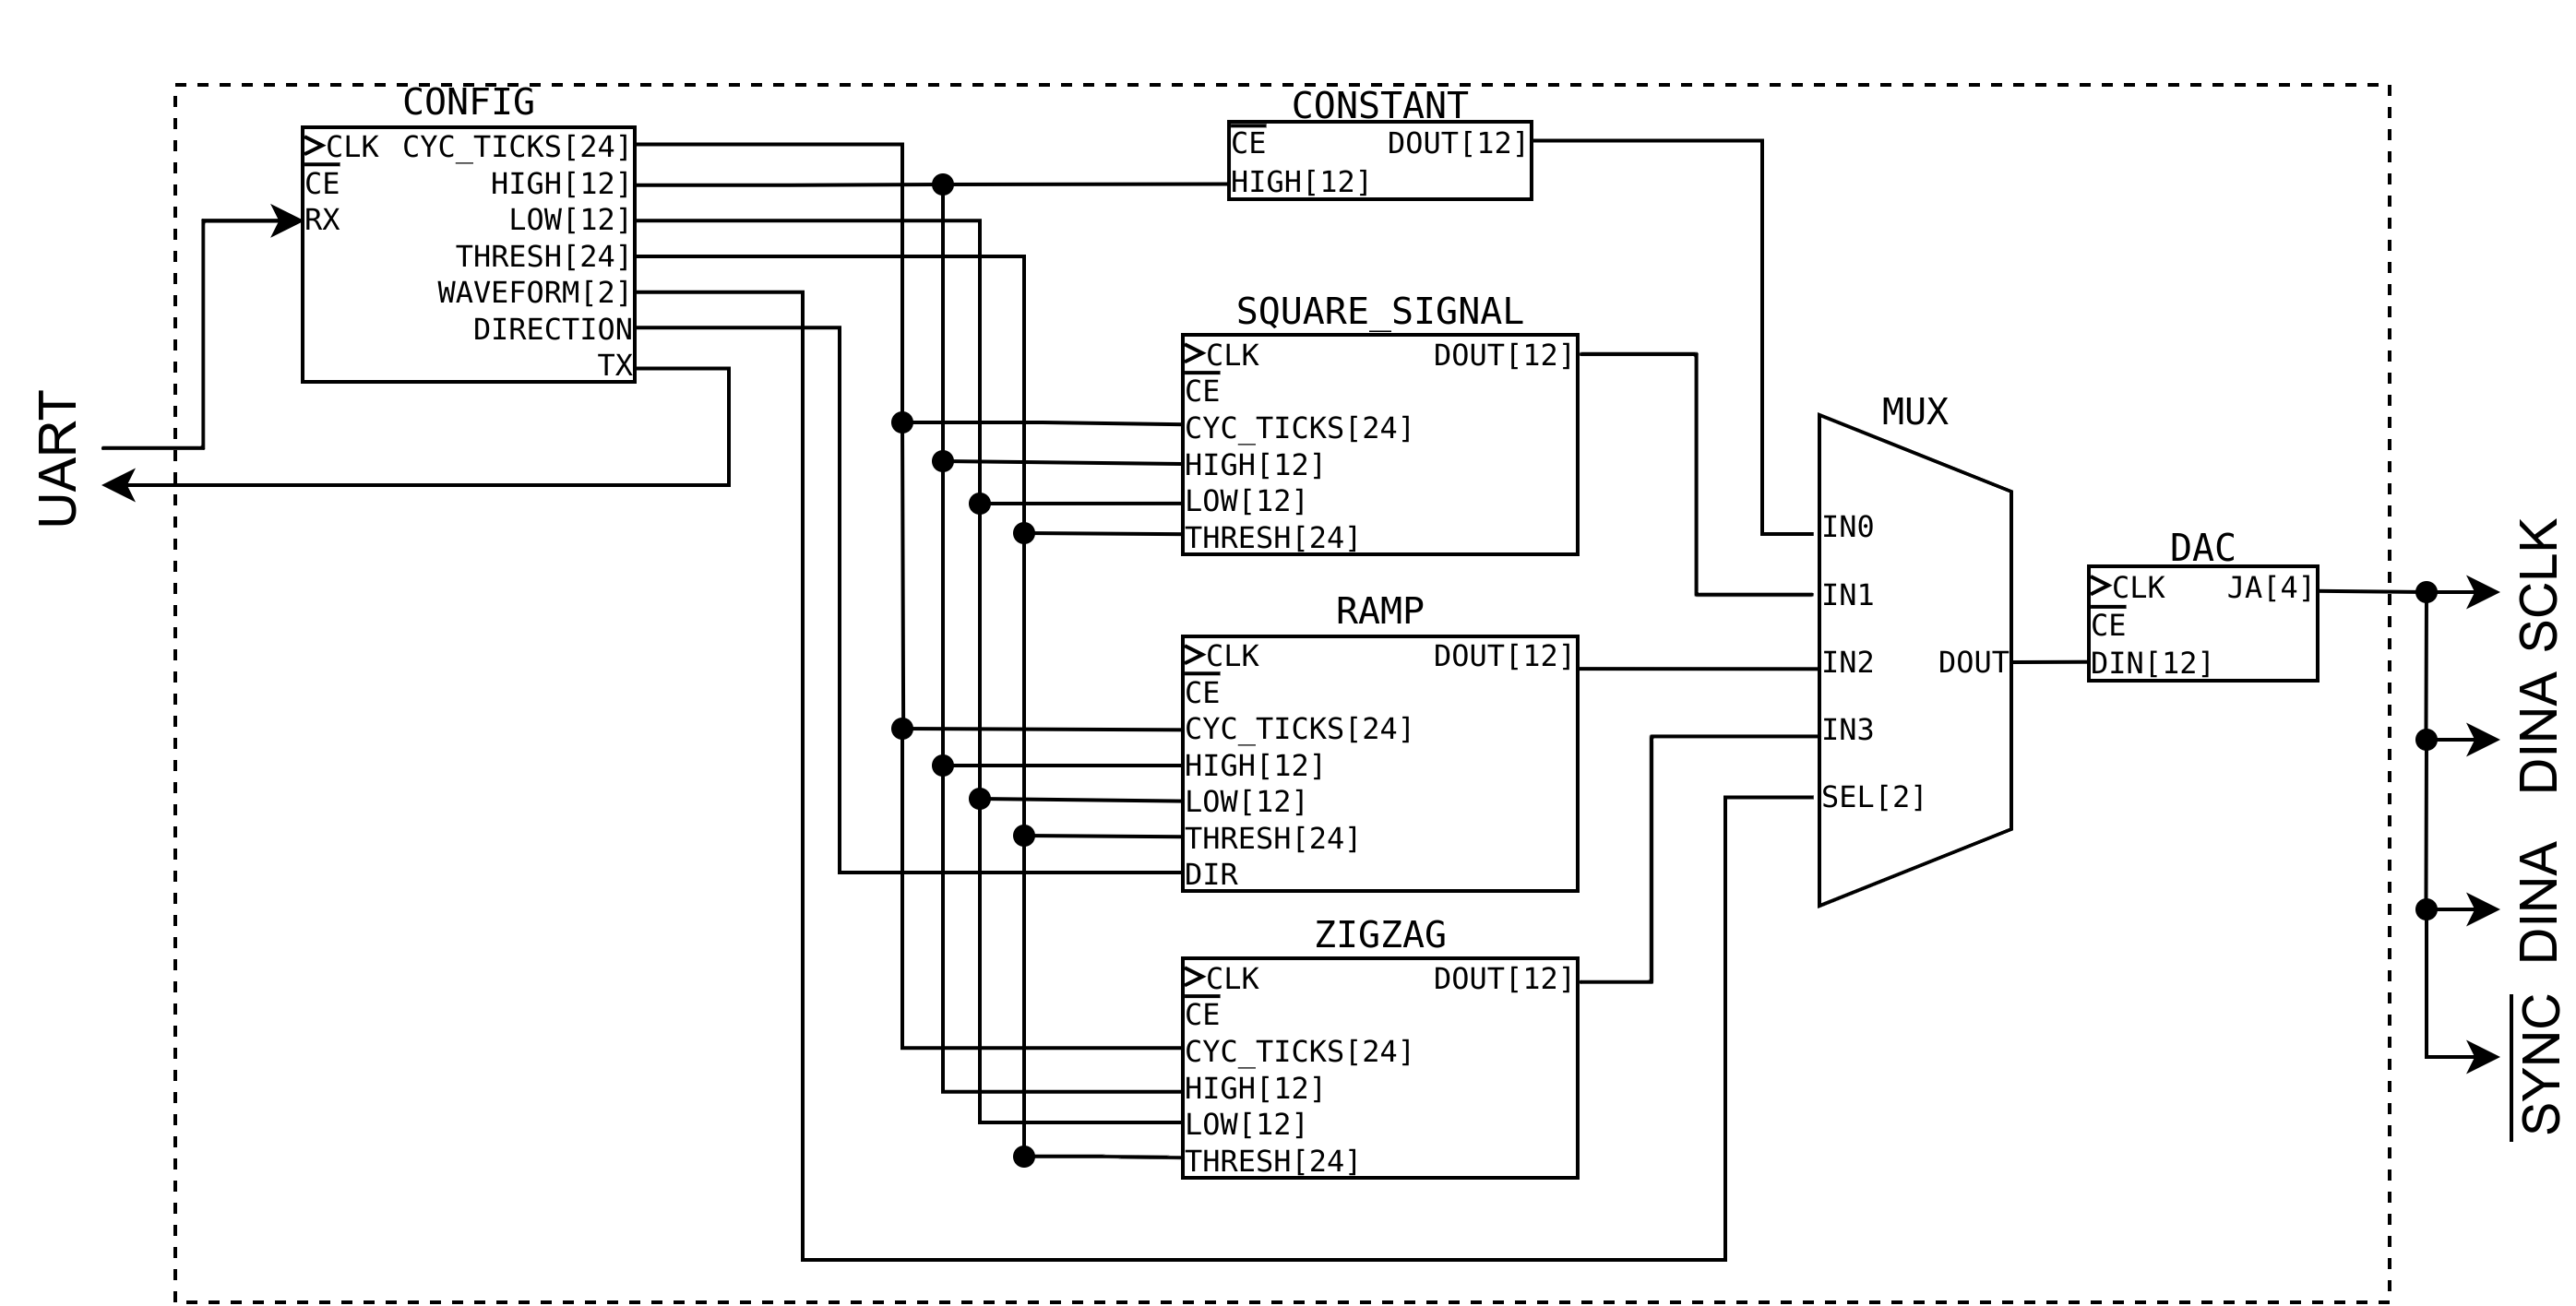
\includegraphics[width=1.0\textwidth, angle=-90, origin=c]{function_generator}
  \caption{Diagramm des Funktionsgenerators. Aus Gründen der Übersichtlichkeit sind die \bit{CLK} Signale und \lowactive{CE} Signale nicht angeschlossen dargestellt. Alle \bit{CLK} Signale sind an den Systemtakt angeschlossen und alle \lowactive{CE} Signale liegen auf Masse.}  \label{Concept:FuncGenDia}
\end{figure}


\chapter{Komponenten}
In diesem Kapitel soll der Aufbau des Funktionsgenerators anhand seiner
digitaltechnischen Komponenten erläutert werden.

\section{Arithmetik}
Der Funktionsgenerator braucht für die richtige Berechnung des Ergebnisses Komponenten, mit deren Hilfe mathematische Operationen ausgeführt werden können.
Zum Addieren, Subtrahieren und Multiplizieren vorzeichenloser Zahlen können die VHDL Standardfunktionen des Datentyps \code{unsigned} verwendet werden.
Darüber hinaus benötigte Funktionen, die über eine eigene Implementierung verfügen, werden im Folgenden vorgestellt.

\subsection{Zähler} \label{Comp:Arith:Count}
Der Zähler bildet die Basiskomponente der Funktionskomponenten. Er eignet sich sehr gut, um die Zeit zu messen, da sich die Zeit seit dem letzten Rücksetzen des Zählers $T_{R}$ immer aus dem Zählstand $N$ und der Taktzeit des Zählers $T_{count}$ berechnen lässt: $T_{R} = N \cdot T_{count}$. So kann durch wiederholtes Rücksetzen des Zählers bei einem bestimmten Zählstand ein zyklischer Funktionsverlauf erstellt werden.
Der Zählstand selbst dient in diesem Fall als diskrete X-Komponente, der dann von der Funktionskomponente ein Y-Wert zugeordnet wird.
Der hier implementierte Zähler kann allerdings schon selbst als Funktionskomponente mit dem Ausgang $o\_count$ für die Funktion $o\_count = inc \cdot N \cdot (-1) ^ {1 - D}, N \in \{0, 1, 2, \dots, max\_ticks\}$ gesehen werden.
Die Komponente besitzt nämlich die Eingänge \code{inc}, \code{D} und \code{max\_ticks}. Diese erfüllen folgende Aufgabe:
\begin{itemize}
\item \code{max\_ticks}: Bit-Vektor, der den maximalen Wert repräsentiert, ab dem der Zähler automatisch zurückgesetzt wird.
Diese Funktion erleichtert es, die Zykluszeit einer Funktion $T_{func}$ als Zeitraum zwischen zwei Rücksetzungen festzulegen: $T_{func} = max_{ticks} \cdot T_{func}$
\item \code{D}: Richtung, in die der Zähler Zählen soll: 0 heißt aufwärts, 1 heißt abwärts
  \item \code{inc}: Bit-Vektor, er repräsentiert das Inkrement, um das der Zähler hoch- bzw. runterzählen soll
\end{itemize}

Der maximale Zählstand ist durch die Anzahl der Stellen von \code{o\_count} beschränkt. Sie kann generisch durch den Wert \code{data\_width} bestimmt werden. \\
Würde es im nächsten Takt dazu kommen, dass der Zählstand größer als \code{max\_ticks} wird (Überlauf), setzt er sich automatisch wieder auf Null zurück.
Würde es im nächsten Takt dazu kommen, dass der Zählstand kleiner als Null wird (Unterlauf), wird der Zähler auf \code{max\_ticks} zurückgesetzt.
Zusätzlich kann der Zähler asynchron auf Null gesetzt werden, wenn der Eingang \code{R} auf 0 gesetzt wird.


\subsection{Teiler} \label{Comp:Arith:Division}
Während beim Multiplizieren, Addieren und Subtrahieren auf Standardfunktionen
zurückgegriffen wird, wird für die Division zweier Binärzahlen eine eigene
Komponente entworfen. Die Gründe hierfür werden in \cref{Comp:Func:ZigZag}
erläutert. \\ % Quelle: https://en.wikipedia.org/wiki/Division_algorithm
Diese Komponente kann die Division des Zählers $Z$ durch den Nenner $N$
lösen, dabei sind $Z$ und $N$ zwei Binärzahlen mit gleicher
Stellenanzahl und ohne Vorzeichen. Das Ergebnis ist der Quotient $Q$ und der Rest $R$. Der Algorithmus, den die Komponente ausführt, ermittelt dabei pro Rechenschritt (d.h. pro Takt) eine Stelle des Ergebnisses.
Er geht den Zähler von der größten bis zur kleinsten Stelle durch und schiebt die immer die aktuelle Stelle $Z(i)$ in den Rest, sodass der neue Rest im binären $R' = R \cdot 2 + Z(i)$ ist.
Immer wenn der Rest größer wird als der Nenner, ist das Ergebnis der Division größer Null, also wird der neue Rest durch Subtraktion mit dem Nenner gebildet: $R'' = R' - N$.
Ist eine Subtraktion möglich, ist $Q$ an dieser Stelle Eins, ansonsten ist $Q$ Null. Der nachfolgende Pseudocode verdeutlicht den Algorithmus noch einmal.
Es gilt dabei aber zu beachten, dass alle Schritte innerhalb der Schleife in einem Takt ausgeführt werden können, da es sich bei der Komponente um eine digitale Schaltung handelt.

\begin{verbatim}
Beginn des Algorithmus
// verhindern, dass durch 0 geteilt wird:
wenn N ungleich 0, dann
    setze Q = 0
    setze R = 0
    zähle i von n - 1 bis 0 runter  // n ist die Anzahl der Bits in N
        schiebe R um 1 Bit nach links
        // letzte Stelle von R wird ite Stelle des Zählers:
        R(0) = Z(i)                    
        wenn R >= N, dann               
            setze R = R - N
            setze Q(i) = 1  // ite Stelle des Quotienten wird 1 
        Ende der bedingten Anweisung
    springe zum Anfang der Schleife
Ende der bedingten Anweisung
Ende des Algorithmus
\end{verbatim}

\section{Takterzeugung}
Da die Einzelkomponenten des Funktionsgenerators in verschiedenen Geschwindigkeiten arbeiten, braucht es Komponenten für das Clock-Management. 
\subsection{Clock-Enable} \label{Comp:Tact:ClkEn}
Um aus dem Systemtakt Takte mit niedrigerer Frequenz zu erzeugen, wird die Komponente \code{SCLK\_ENABLE} verwendet.
Der Takt wird geteilt, indem ein sogenanntes Enable-Signal \code{SCLK\_EN} erzeugt wird, das die jeweils nte steigende Flanke des Systemtakts mit \code{low} maskiert.
Der Eingang \code{CE} der Komponente, die im erzeugten Takt arbeiten soll, wird an \code{SCLK\_EN} angeschlossen, so dass die Komponente nur dann aktiv ist, wenn eine steigende Flanke detektiert wurde und \code{CE=0} anliegt.
Das Timingdiagram in Abbildung \cref{Comp:Tact:ClkEn:Timing} verdeutlicht, auf welche Taktzyklen die angeschlossene Komponente reagiert.
Der große Vorteil dieser Methode liegt darin, dass jede Komponente weiterhin direkt an den Systemtakt angeschlossen ist und dieser somit nicht durch zwischengeschaltete Komponenten verzögert wird.
\vfill
\begin{tikztimingtable} 
  CLK                             & H 9{2L 2H} L    \\
  $\overline{\mbox{CLK\_Enable}}$ & H 3{4L 8H} L    \\
  aktive Zyklen                   & 3L 3{2H 10L} L  \\
  \extracode
  \tablerules
  \begin{pgfonlayer}{background}
    \foreach \n in {1, ..., 8}
    \draw [help lines] (A\n) -- (B\n);
  \end{pgfonlayer}

\end{tikztimingtable}
\captionof{tikztimingtable}{Beispielhaftes Timing-Diagramm. Jeder vierte Taktzyklus wird durch \lowactive{CLK\_Enable} aktiviert.} \label{Comp:Tact:ClkEn:Timing}


\section{Funktionen}   \label{Comp:Func}
Die Herzstücke des Funktionsgenerators bilden seine Funktionskomponenten.
An ihren Ausgängen liegen die von ihnen berechneten Werte an, von denen einer zum in \cref{Comp:DAC} beschriebenen DAC-Konverter per Multiplexer weitergeleitet wird.
Bis auf die Konstante verfügen alle Komponenten, neben den üblichen \code{CLK} und \lowactive{CE} Eingängen, über folgende Anschlüsse:

\begin{itemize}
\item \code{cyc\_ticks}: Eingang, dieser Bit-Vektor legt die Periodendauer einer Funktionskomponente fest.
\item \code{high}: Eingang, dieser Bit-Vektor legt den maximal erreichbaren Wert des Komponentenausgangs fest.
\item \code{y\_out}: Ausgang, der digitale Funktionswert, der zum DAC geschickt wird
\end{itemize}

Alle Komponenten außer der Konstante verfügen über einen Zähler und eine Clock-Enable-Komponente, die die Geschwindigkeit des Zählers steuert.
Darüber hinaus können sie noch über drei generische Größen konfiguriert werden:

\begin{itemize}
\item \code{data\_width}: legt die Bitbreite des \code{high}, \code{low} und \code{y\_out} Signals fest.
Bei allen Funktionen ist diese auf zwölf eingestellt, da es sich beim DAC-Wandler um einen 12-Bit-Konverter handelt.
\item \code{clk\_width}: legt die Bitbreite von \code{cyc\_ticks} und \code{thresh} fest.
  Diese muss größer als \code{data\_width} sein.
  Die \code{clk\_width} legt fest, welche Periodendauer maximal erreicht werden kann, da sie den maximal möglichen Zählerstand begrenzt.
\item \code{clk\_ticks\_per\_count}: Dies ist der Teilungsfaktor zwischen dem angelegten Takt und dem Takt, mit dem der interne Zähler hochzählt.
\end{itemize}


\subsection{Konstante}   \label{Comp:Func:Const}
Die konstante Funktion ist die einfachste der vier Funktionskomponenten.
Sie gibt lediglich den an ihr anliegenden high-Wert auf ihrem Ausgang aus.
Sie verfügt darüber hinaus noch über den Eingang \lowactive{CE}, der bewirkt, dass der Ausgang asynchron auf 0 gesetzt wird.
\subsection{Rechteck}   \label{Comp:Func:Square}
Die Rechteckfunktion verfügt über einen Eingang \code{thresh}, der mit dem Stand des internen Zählers verglichen wird.
Ist der Zähler größer als \code{thresh}, so wird der Ausgang auf den Wert \code{high} gesetzt, ansonsten ist er auf den Wert \code{low} eingestellt.
Der \code{low}-Wert liegt als weiteres Eingangssignal an.

\subsection{Zick-Zack}  \label{Comp:Func:ZigZag}


\subsection{Rampe} \label{Comp:Func:Ramp}

\section{Konfigurationsschnittstelle}
Die Konfigurationsschnittstelle \code{CONFIG\_INTERFACE} besteht aus einer
UART-Schnittstelle, über die der Datenaustausch zwischen Benutzer und
Funktionsgenerator erfolgt, sowie der Instruktionsauswertung, die die
empfangenen UART-Signale in Konfigurationsbefehle übersetzt.
\subsection{UART-Schnittstelle}
Die UART-Schnittstelle beruht auf dem
\textbf{U}niversal-\textbf{A}synchronous-\textbf{R}ceiver-\textbf{T}ransmission-Protokoll.
Das Protokoll ermöglicht es, byteweise serielle Daten zu verschicken und zu
empfangen. Hierfür reichen zwei Drähte aus, die jeweils eins der beiden Signale
RX (Receive) und TX (Transmit) transportieren. Zum Start der Kommunikation wird
die RX Leitung vom Sender von high auf low gezogen. Der Empfänger detektiert
dieses Startsignal und fängt an, die nachfolgenden acht Bits zu einem Byte
zusammenzusetzen.
Wurde ein Byte übertragen, muss mindestens ein Stop-Bit folgen, bei dem die Receive Leitung des Empfängers auf
High liegt. Darauf kann, je nach Implementierung, noch ein Stop-Bit sowie
ein Paritätsbit folgen. Da es zwischen dem Sender und Empfänger kein synchrones
Taktsignal gibt, ist es wichtig, dass ihre Sende- und Empfangsfrequenz gleich
ist. Diese Frequenz ist die sogenannte Baudrate. Im Funktionsgenerator ist sie
auf 115200 Bits / s festgelegt. \\
Die im Generator verwendete Schnittstelle wurde,
um den Arbeitsaufwand zu verringern, aus einer Vorlage übernommen (Quelle). Sie
beinhaltet sowohl eine Empfänger- als auch eine Sender-Komponente. Es gibt
folgende Eingangssignale:
\begin{enumerate}
\item \code{CLK}: Eingang, gibt die Taktfrequenz der Komponente vor
\item \code{CE}: Eingang, ''chip-enable``-Signal, aktiviert die Komponente wenn es auf
  low gesetzt wird
\item \code{reset}: Eingang, die Schnittstelle wird auf den Initialisierungszustand zurückgesetzt und die aktuelle Übertragung bzw. aktuelle Empfangsprozesse werden abgebrochen.

\item \code{tx}: Ausgang, Das von der Schnittstelle versendete TX-Signal 
  \item \code{tx\_start}: Eingang, wenn \code{tx\_start} auf high gesetzt wird, wird mit der
    Übertragung von \code{data\_in} begonnen
\item \code{data\_in}: Eingang, ein 8-Bit breites Signal, dass das zu versendende Byte enthält.

\item \code{rx}: Eingang, das von der Schnittstelle empfangene RX-Signal
\item \code{data\_out}: Ausgang, ein 8-Bit breites Signal, dass das zuletzt von der Schnittstelle empfangene Byte beinhaltet.
\item \code{rx\_uart\_rdy}: Ausgang, dieses Signal zeigt an, wenn ein komplettes Byte
  empfangen wurde und bereit ist, gelesen zu werden.
\end{enumerate}
  
\subsection{Instruktionsauswertung}

\section{DAC-Konverter} \label{Comp:DAC}
\subsection{DAC-Kanal}


% \chapter{Clocking}

\begin{figure} \centering
  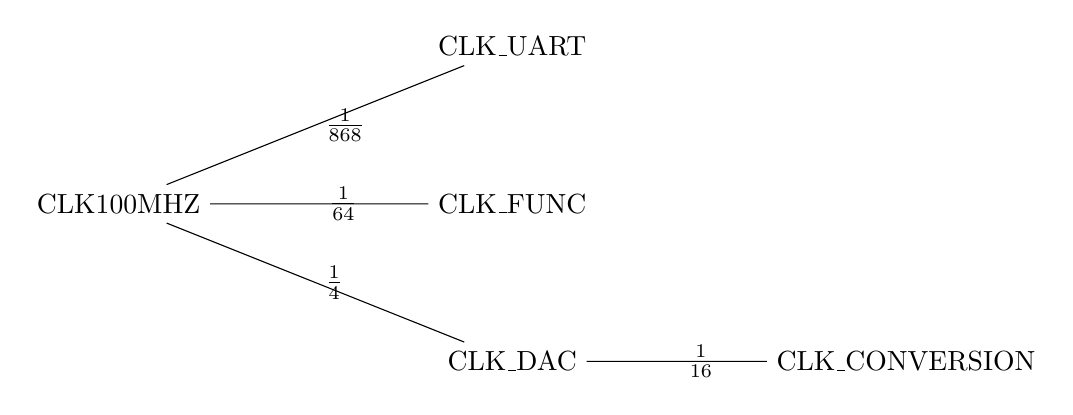
\begin{tikzpicture} 
    \node {CLK100MHZ}[grow=east, sibling distance=2cm, level distance=5cm]
    child {node {CLK\_DAC}
      child {node {CLK\_CONVERSION}
      edge from parent node [right] {$\frac{1}{16}$}}
      edge from parent node [right] {$\frac{1}{4}$}}
    child {node {CLK\_FUNC}
      edge from parent node [right] {$\frac{1}{64}$}}
    child {node {CLK\_UART}
      edge from parent node [right] {$\frac{1}{868}$}};
  \end{tikzpicture} 
  \caption{Clock-Tree} \label{clk:clocktree}
\end{figure}


% \input{Benchmark}
%Schluss
% \chapter{Fazit}
Es wurde erfolgreich ein digitaler Funktionsgenerator auf dem Basys 3 Board implementiert.
Dieser kann vier verschiedene Funktionen ausgeben und über eine UART Schnittstelle konfiguriert werden. \\
Das dem Generator zugrundeliegende Konzept und das Zusammenspiel der Einzelkomponenten wurde erläutert.
Auch das interne Clock-Management wurde geschildert. \\
Die theoretischen Grenzen der Auflösung und der Frequenz wurden aufgezeigt. 
Darüber hinaus konnte seine Funktionstüchtigkeit in dem Frequenzbereich 0,1 Hz bis 10 kHz bewiesen werden.
Alle Frequenzen unterhalb von $f_{min}$ führen zu einer höheren Ausgangsfrequenz als der gewünschten.
Zwischen 10 kHz und $f_{max}$ wird das Ausgangssignal unsauber und oberhalb von $f_{max}$ ist eine zuverlässige Ausgabe nicht mehr möglich.
Warum das Signal oberhalb von 10 kHz derart ungenau wird, konnte teilweise erklärt werden.
Hier sollten jedoch weitere Untersuchungen angestrebt werden, um die Fehlerursache vollständig zu klären.\\
Die Ausgangsspannung entspricht nicht ganz der eingestellten Spannung.
Eine bessere Referenzspannung könnte aber für einen saubereren Ausgangspegel sorgen.
Allerdings wurde die Korrektheit des Ausgangspegels bis jetzt nur für die Spannung 0 und 3,3 V untersucht.
Um ein vollständigeres Bild der Genauigkeit zu bekommen, sind weitere Nachforschungen nötig.\\
Es wurde gezeigt, dass die Konfiguration per UART-Schnittstelle funktioniert.
Außerdem wurde der Befehlssatz des Funktionsgenerators dokumentiert, sodass andere.

% \chapter{Ausblick}
Durch die Implementation der Funktionskomponenten als Bausteine ist es relativ leicht, die möglichen Funktionsformen zu erweitern.
Z.B. könnte noch eine Sinusfunktion hinzugefügt werden.
Theoretisch könnte auch ein nicht-periodisches Signal, wie ein zeitversetzter Sprung hinzugefügt werden.\\
Außerdem kann die UART-Schnittstelle noch um weitere Features ergänzt werden.
Es wäre beispielsweise denkbar, die gegenwärtigen Funktionsparameter über den Transmitter an den User zurück zu schicken, sodass dieser sie leichter kontrollieren kann.
Dazu müsste auch die Konfigurationsschnittstelle um Befehle zur Rückgabe der Funktionsparameter erweitert werden. \\
Darüber hinaus könnte auch noch der zweite Kanal auf dem DAC-Konverter genutzt werden um zwei verschiedene Signale gleichzeitig auszugeben. \\
Abschließend fehlt auch noch der Test in einer realen Anwendung, z.B. einem Trigger für eine Fotokamera, die in einer bestimmten Frequenz Bilder aufnehmen soll.

\end{document}
